\documentclass[a4paper, 16pt]{article}
\usepackage[UTF8]{ctex}
\usepackage{geometry}
\usepackage{graphicx}
\usepackage{setspace}
\usepackage{float}
\usepackage{listings}
\usepackage{xcolor}
\lstset{
    numbers=left, 
    numberstyle= \tiny, 
    keywordstyle= \color{ blue!70},
    commentstyle= \color{red!50!green!50!blue!50}, 
    frame=shadowbox, % 阴影效果
    rulesepcolor= \color{ red!20!green!20!blue!20} ,
    escapeinside=``, % 英文分号中可写入中文
    xleftmargin=2em,xrightmargin=2em, aboveskip=1em,
    framexleftmargin=2em
} 
\geometry{left = 1.0 cm, right = 1.0cm, top = 2.0cm, bottom = 2.0cm	}
\title{编译原理第二章(二)}
\author{李鹏辉}

\begin{document}
\maketitle
1. (2.8.1)按照类IF,为FOR语句定义一个类FOR. \\

\centerline{$for ( expr_1 ; expr_2 ; expr_3 ) stmt;$}
\centerline{$expr_1; while( expr_2) \{stmt; expr_3; \}$}
\begin{figure}[H]
\centering
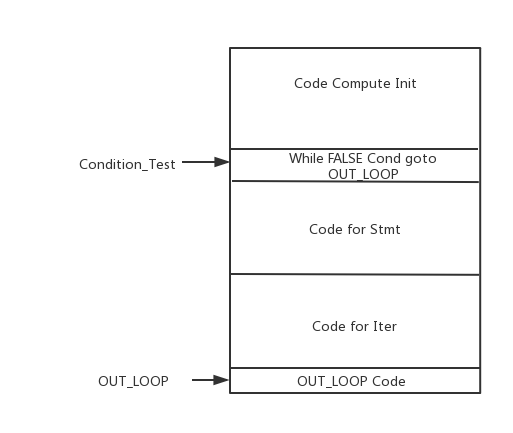
\includegraphics[scale=0.6]{chapter2_hw2_1}
\caption{Graph for FOR statement}
\end{figure}

\lstset{language=C}
\begin{lstlisting}
class FOR extends Stmt{
	Expr Init; Expr Cond; Expr Iter; Stmt S;
	public FOR(Expr e1, Expr e2, Expr e3, Stmt s1){
		Init = e1; Cond = e2; Iter = e3; S = s1; 
		Cond_Test = newlabel(Cond); 
		OUT_LOOP = newlabel();
	}
	
	public void gen(){
		Expr t0 = Init.gen();
		Expr t1 = t0.rvalue();
		emit("compute Init", t1.toString());
		Expr t2 = Cond.rvalue();
		emit("ForCondFalse" + t2.toString() + "goto" + OUT_LOOP);
		S.gen();
		Iter.gen();
		emit("goto" + Cond_Test);
		emit(OUT_LOOP);
	}
}
\end{lstlisting}

\end{document}